\documentclass[10pt]{standalone}
\usepackage[utf8]{inputenc}
\usepackage{pgf,tikz,pgfplots}
\pgfplotsset{compat=1.15}
\usepackage{mathrsfs}
\usetikzlibrary{arrows}
\pagestyle{empty}
\begin{document}

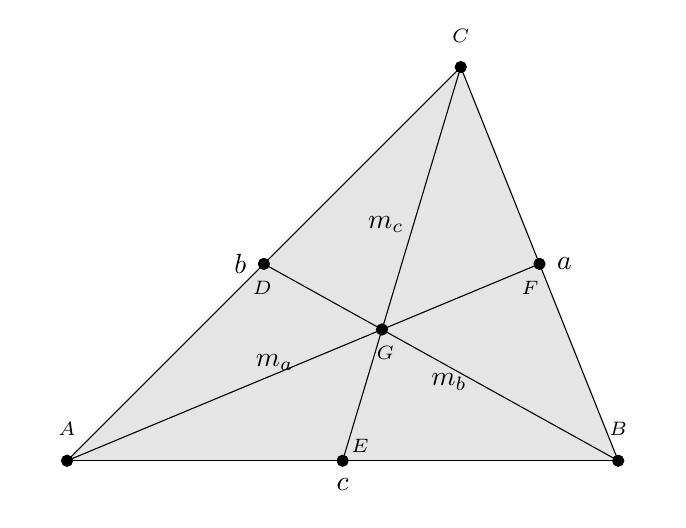
\begin{tikzpicture}[line cap=round,line join=round,>=triangle 45,x=1.0cm,y=1.0cm]

\clip(-0.5,-0.5) rectangle (7.5,5.5);
\fill[line width=2.pt,color=black,fill=black,fill opacity=0.10000000149011612] (0.,0.) -- (7.,0.) -- (5.,5.) -- cycle;
\draw  (0.,0.)-- (7.,0.)node [midway,below=0.1cm] {$c$};
\draw  (7.,0.)-- (5.,5.)node [midway,right=0.1cm] {$a$};
\draw  (5.,5.)-- (0.,0.)node [midway,left=0.1cm] {$b$};
\draw  (0.,0.)-- (6.,2.5)node [pos=0.5,left] {$m_a$};
\draw  (7.,0.)-- (2.5,2.5)node [pos=0.4,left] {$m_b$};
\draw  (3.5,0.)-- (5.,5.)node [pos=0.6,left] {$m_c$};
\begin{scriptsize}
\draw [fill=black] (0.,0.) circle (2.0pt);
\draw (0.0,0.4) node {$A$};
\draw [fill=black] (7.,0.) circle (2.0pt);
\draw (7.0,0.4) node {$B$};
\draw [fill=black] (5.,5.) circle (2.0pt);
\draw (5.0,5.4) node {$C$};
\draw [fill=black] (2.5,2.5) circle (2.0pt);
\draw (2.48,2.19) node {$D$};
\draw [fill=black] (3.5,0.) circle (2.0pt);
\draw (3.72,0.19) node {$E$};
\draw [fill=black] (6.,2.5) circle (2.0pt);
\draw (5.88,2.19) node {$F$};

\draw [fill=black] (4.,1.6666666666666667) circle (2.0pt);
\draw (4.04,1.37) node {$G$};
\end{scriptsize}
\end{tikzpicture}
\end{document}